% flashcards-title: One vector in two coordinate systems
% flashcards-desc: One fixed arrow is overlaid by a solid x-y frame and a rotated dashed x-prime-y-prime frame.
\documentclass[border=7pt]{standalone}
\def\pgfsysdriver{pgfsys-dvisvgm.def}
\usepackage{tikz}
\usetikzlibrary{arrows.meta,positioning,shapes.geometric}
\definecolor{mechInk}{HTML}{172033}
\definecolor{mechBlue}{HTML}{155EEF}
\definecolor{mechOrange}{HTML}{B54708}
\definecolor{mechPale}{HTML}{E8F0FF}
\definecolor{mechGray}{HTML}{667085}
\definecolor{mechLight}{HTML}{D0D5DD}
\tikzset{
  every picture/.style={font=\sffamily\large, text=mechInk},
  mech box/.style={draw=mechInk, line width=1.2pt, rounded corners=4pt,
    fill=white, align=center, minimum height=14mm, inner xsep=5mm},
  mech primary/.style={draw=mechBlue, line width=2.2pt},
  mech secondary/.style={draw=mechOrange, line width=2.2pt, dashed},
  mech guide/.style={draw=mechGray, line width=0.9pt, dashed},
  mech arrow/.style={-{Stealth[length=3.2mm,width=2.4mm]},
    draw=mechInk, line width=1.4pt, line cap=butt},
  mech axis/.style={draw=mechInk, line width=1.2pt},
  mech tick/.style={draw=mechInk, line width=1pt}
}

\begin{document}
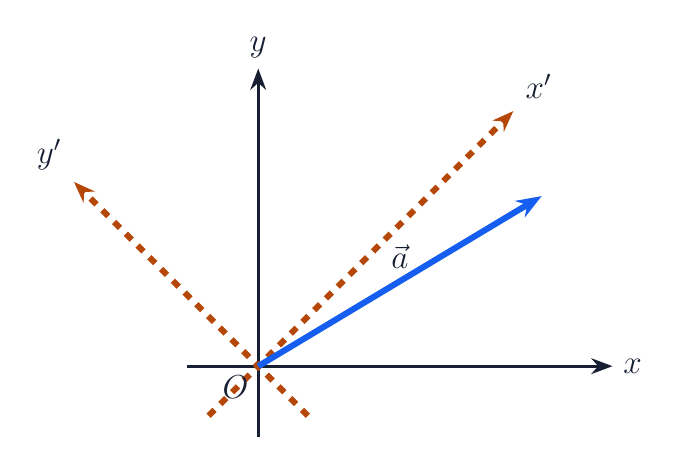
\begin{tikzpicture}[x=0.9cm,y=0.9cm]
  \draw[mech axis,-{Stealth[length=2.7mm,width=2mm]}] (-1,0) -- (5,0) node[right] {$x$};
  \draw[mech axis,-{Stealth[length=2.7mm,width=2mm]}] (0,-1) -- (0,4.2) node[above] {$y$};
  \draw[mech secondary,-{Stealth[length=2.7mm,width=2mm]},line cap=butt] (-0.7,-0.7) -- (3.6,3.6) node[above right] {$x'$};
  \draw[mech secondary,-{Stealth[length=2.7mm,width=2mm]},line cap=butt] (0.7,-0.7) -- (-2.6,2.6) node[above left] {$y'$};
  \draw[mech primary,-{Stealth[length=3.2mm,width=2.4mm]},line cap=butt] (0,0) -- (4,2.4) node[midway,above] {$\vec a$};
  \node[below left] at (0,0) {$O$};
\end{tikzpicture}
\end{document}
